%!program = pdflatex

%\documentclass{article}
\documentclass[12pt]{article}
%\documentclass [12pt,a4paper]{report}

\usepackage{array}
%\usepackage[english]{babel}


% General packages for math and document geometry
\usepackage{geometry}
\usepackage{amsmath} %ftp://ftp.ams.org/ams/doc/amsmath/short-math-guide.pdf
\usepackage{amsthm}
\usepackage{amssymb}

%\usepackage[latin1]{inputenc}
%\usepackage[english]{babel}

\usepackage[estonian, english]{babel} %mainlanguage should be english & chance to estonian if needed...
\usepackage[applemac]{inputenc}
\usepackage[T1]{fontenc}

%\usepackage[latin5]{inputenc}
%\usepackage[T1]{fontenc}
%\usepackage[english, estonian]{babel}

%\usepackage[estonian]{babel}
%\usepackage[T1]{fontenc} % t�pit�hed

%\usepackage{graphics}
%\usepackage[mathscr]{eucal}
\geometry{a4paper}

\usepackage{tikz}
\usetikzlibrary{matrix}

\usepackage{tabu} %wide lines in tables

\usepackage{graphicx}
\usepackage{xspace}

\graphicspath{{figures/}}

%%%% code printing
\usepackage{listings}
\usepackage{color}
 
\definecolor{dkgreen}{rgb}{0,0.6,0}
\definecolor{gray}{rgb}{0.5,0.5,0.5}
\definecolor{mauve}{rgb}{0.58,0,0.82}

\lstset{ 
  %language=python,                % the language of the code
  language=C++,
  basicstyle=\footnotesize,           % the size of the fonts that are used for the code
  %numbers=left,                   % where to put the line-numbers
  %numberstyle=\footnotesize,          % the size of the fonts that are used for the line-numbers
  numberstyle=\tiny\color{gray}, 
  stepnumber=1,                   % the step between two line-numbers. If it's 1, each line 
                                  % will be numbered
  numbersep=5pt,                  % how far the line-numbers are from the code
  backgroundcolor=\color{white},      % choose the background color. You must add \usepackage{color}
  showspaces=false,               % show spaces adding particular underscores
  showstringspaces=false,         % underline spaces within strings
  showtabs=false,                 % show tabs within strings adding particular underscores
  frame = lines,
  %frame=single,                   % adds a frame around the code
  rulecolor=\color{black},		% if not set, the frame-color may be changed on line-breaks within not-black text (e.g. commens (green here))
  tabsize=2,                      % sets default tabsize to 2 spaces
  captionpos=b,                   % sets the caption-position to bottom
  breaklines=true,                % sets automatic line breaking
  breakatwhitespace=false,        % sets if automatic breaks should only happen at whitespace
  %title=\lstname,                   % show the filename of files included with \lstinputlisting;
                                  % also try caption instead of title
                                 % also try caption instead of title
  keywordstyle=\color{blue},          % keyword style
  commentstyle=\color{dkgreen},       % comment style
  stringstyle=\color{mauve},         % string literal style
  escapeinside={\%*}{*)},            % if you want to add a comment within your code
  morekeywords={*,game, fun}               % if you want to add more keywords to the set
}



\usepackage[ruled, vlined, linesnumbered]{algorithm2e}
\usepackage{proof} % http://logicmatters.net/resources/ndexamples/proofsty3.html <= writing type rules => use semantic::inference
\setlength{\inferLineSkip}{4pt}
\usepackage{semantic} %ftp://tug.ctan.org/tex-archive/macros/latex/contrib/semantic/semantic.pdf
\def\predicatebegin #1\predicateend{$\Gamma \vdash #1$}


\usepackage{todonotes}
\usepackage{hyperref}
\usepackage[all]{hypcap}

%%Prover
\newcommand{\proveit} {ProveIt\xspace}

\newcommand{\tab}{\hspace*{2em}}
\newcommand{\Gd} {\ensuremath{\Gamma \vdash}\xspace}
\newcommand{\BBox} {\ensuremath{\blacksquare}\xspace}
\newcommand{\TODO}{\todo[inline]}
\newcommand{\typeG} {\ensuremath{\mathsf{type_G}}\xspace}
\newcommand{\typeF}[1] {\ensuremath{\mathsf{type_{#1}}}\xspace}

\newtheorem{theorem}{Theorem}


%using in the algorithms
\SetKw{True}{true}
\SetKw{False}{false}
\SetKwData{maxType}{maxType}
\SetKwData{minType}{minType}
\SetKwData{typeMax}{Max}
\SetKwData{typeMin}{Min}
\SetKwData{typeInt}{Int}
\SetKwData{typeRat}{Rat}
\SetKwData{Defined}{Defined}
\SetKwData{Var}{var}
\SetKwData{Type}{type}
\SetKwData{Left}{left}
\SetKwData{Right}{right}
\SetKwFunction{Error}{errorMessage}
\SetKwFunction{updateMinType}{updateMinType}
\SetKwFunction{updateMaxType}{updateMaxType}
\SetKwFunction{parseExpression}{parseExpression} 
\SetKwFunction{parseStatement}{parseStatement}
\SetKwFunction{typeChecking}{typeChecking}

\SetKwFunction{LCA}{LCA}


\SetKwFunction{adv}{\ensuremath{\backslash adv}}
\SetKwFunction{gameIf}{if}
\SetKwFunction{Game}{game g}
\SetKwFunction{Fun}{fun f}



\newcommand{\opExp}{\ensuremath{^\wedge}\xspace} %\tiny^\wedge - is better but copy-paste is bad...
\newcommand{\opDiv}{\ensuremath{\backslash \mathsf{div}}\xspace} %should use the way the renderer does it...
%\newcommand{\codeExample}[1] {\begin{lstlisting} \\ a := b \\ \end{lstlisting}}


\newenvironment{game}[1]
{\begin{aligned} &\hspace{0.3em}#1\\ &\left[\begin{aligned}}{\end{aligned}\right.\end{aligned}}


%%% BEGIN DOCUMENT
\begin{document}

%\listoftodos


%\title{Type Inference for a Cryptographic Protocol Prover Tool}

%\author{Tiina Turban \\ University of Tartu}
%\date{November 18, 2011} 

%\maketitle

% BEGIN TITLE PAGE
\thispagestyle{empty}
\begin{center}

\large
UNIVERSITY OF TARTU\\[2mm]
\uppercase{Faculty of Mathematics and Computer Science}\\[2mm]
Institute of Computer Science\\
%Specialty of Computer Science\\[2mm]

%\vspace*{\stretch{5}}
\vspace{25mm}

\Large Tiina Turban

\vspace{4mm}

\huge Type Inference for a Cryptographic Protocol Prover Tool

%\vspace*{\stretch{7}}
\vspace{20mm}

\Large Bachelor's Thesis (6 ECTS)

\end{center}

\vspace{2mm}

\begin{flushright}
 {
 \setlength{\extrarowheight}{5pt}
 \begin{tabular}{r l} 
  \sffamily Supervisor: & \sffamily Liina Kamm, MSc \\
  \sffamily Supervisor: & \sffamily Sven Laur, PhD
 \end{tabular}
 }
\end{flushright}

%\vspace*{\stretch{3}}
\vspace{10mm}

{\noindent Author: .................................................................................... ``.....'' ..........\hskip16pt 2012}
\vspace{2mm}

{\noindent Supervisor: ............................................................................... ``.....'' ..........\hskip16pt 2012}

\vspace{2mm}

{\noindent Supervisor: ............................................................................... ``.....'' ..........\hskip16pt 2012}

\vspace{8mm}

{\noindent Allowed to defence}

{\noindent Professor: ................................................................................. ``.....'' ..........\hskip16pt 2012}

\vfill
\centerline{Tartu 2012}

% END TITLE PAGE

\tableofcontents

\pagebreak


\newpage
\section{Introduction}

\TODO{What is it in simple terms (title)?}
\TODO{Why should anyone care?}
\TODO{What was my contribution?} 
\TODO{What you are doing in each section (a sentence or two per section)}

Tip: if it's hard for you to start writing, then try to split it to smaller parts, e.g. if the title is "Type Inference for a Cryptographic Protocol Prover Tool" then the "What is it" can be divided into "what is type inference", "what is cryptographic protocol" and "what is the prover tool". These three can also be split to smaller parts etc.





\newpage
\section{Title of Section 2} 
\TODO{Short description of what this section is about}


\subsection{Title of Subsection 1}

Some text...

\subsubsection{Title of Subsubsection 1}

Some text...

\subsubsection{Title of Subsubsection 2}

Some text...



\subsection{Title of Subsection 2} 

Rule: If you divide the text into subsections (or subsubsections) then there has to be at least two of them, otherwise do not create any. 

Tip: You can also use paragraphs, e.g.
\paragraph{Type rules for integers.} Some text ...

\paragraph{Type rules for rational numbers.} Some text here too...





\subsection{How to use references} \label{sec:using_ref}

Tip: Use label and ref to make sure you are always referring to the the correct figure, table or section even if you rearrange them (see Section~\ref{sec:using_ref}).



Example: Game-based proving is a way to analyse security of a cryptographic protocol~\cite{GameB_1, GameB_2}. There are automatic provers, such as {CertiCrypt\-}~\cite{certicrypt} and ProVerif~\cite{proVerif}.

Tip: Jabref (\url{http://jabref.sourceforge.net/}) might be a helpful tool to use.

Tip: Many articles have BibTeX reference ready and you can just copy-paste.



\newpage
\section{How to add figures and pictures to your thesis}


Here are a few examples of how to add figures or pictures to your thesis (see Figures~\ref{fig:fnCompModel}, \ref{fig:game-based_proofs}, \ref{fig:proveit_screenshot}).

Rule: All the figures, tables and extras in the thesis have to be referred to somewhere in the text.



\begin{figure} [ht] %try to place the figure here (next option top of the page) 
\begin{center}
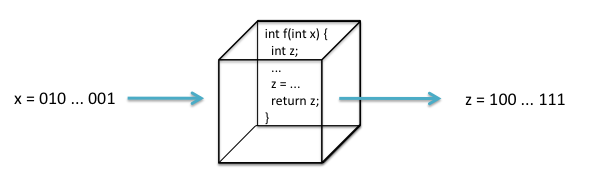
\includegraphics[width=0.8\textwidth]{computational_model_function}
\caption{The title of the Figure}
\label{fig:fnCompModel}
\end{center}
\end{figure}



\begin{figure} [!ht] %if [h] doesn't work, we can force with !
\begin{center}
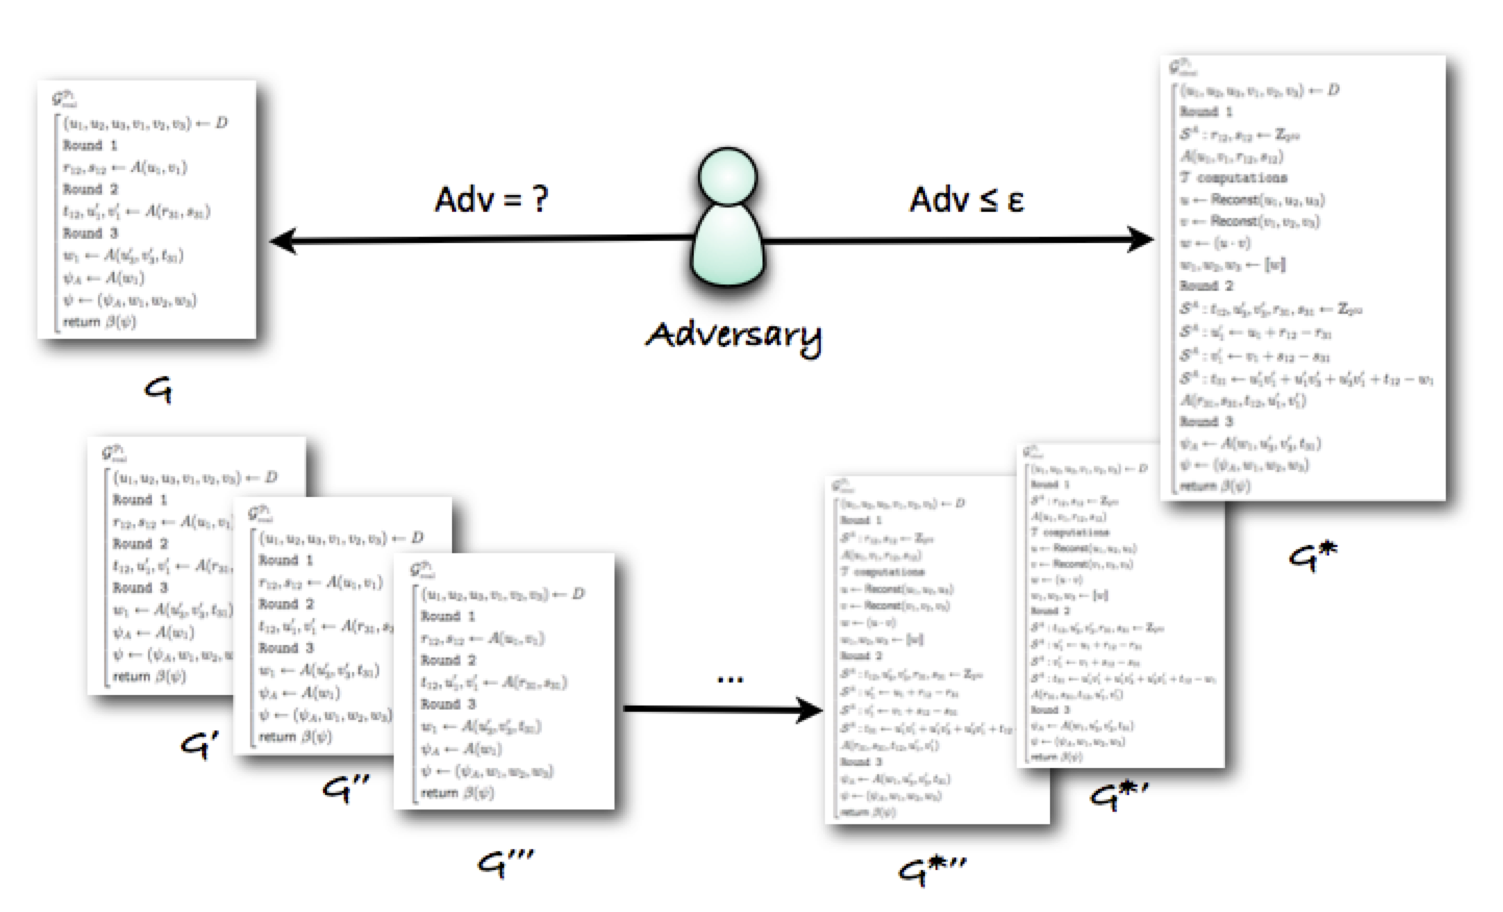
\includegraphics[width=\textwidth]{game-based_proofs}
\caption{Refer if the figure is not yours~\cite{kamm12}}
\label{fig:game-based_proofs}
\end{center}
\end{figure}


\begin{figure} [ht]
\begin{center}
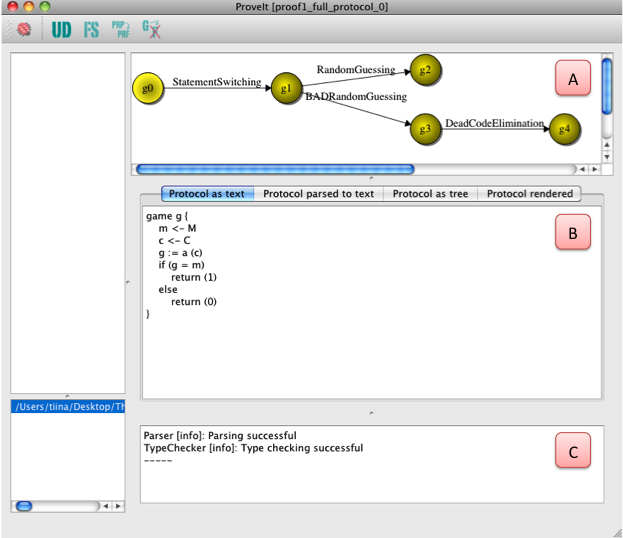
\includegraphics[width=\textwidth]{proveit_screenshot}
\caption{Screenshot of \proveit}
\label{fig:proveit_screenshot}
\end{center}
\end{figure}

Tip: If you add a screenshot then labeling the parts might help make the text more understandable (panel C vs bottom left part), e.g.
 
Example: A screenshot of \proveit can be seen on Figure~\ref{fig:proveit_screenshot}. The user first enters the pseudocode of the initial game in panel B. \proveit also keeps track of all the previous games showing the progress on a graph seen in panel A.


\begin{figure} [!ht]
\begin{tabular}{c c}

\begin{minipage}{0.45\textwidth}
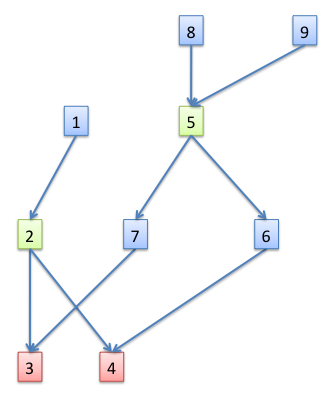
\includegraphics[width=\textwidth]{LCA_2_solutions}
\end{minipage}

&
\begin{minipage}{0.55\textwidth}
\centering
\begin{tabular}{ l | l |}
	Node & Decendants \\ \hline
  1 & 2, 3, 4 \\ \hline
  2 & 3, 4 \\ \hline
  3 & \\ \hline
  4 & \\ \hline
  5 & 3, 4, 6, 7 \\ \hline
  6 & 4 \\ \hline
  7 & 3 \\  \hline
  8 & 3, 4, 5, 6, 7\\ \hline
  9 & 3, 4, 5, 6, 7\\ \hline
\end{tabular}

\end{minipage}

\end{tabular}

\caption{Example how to put two figures parallel to each other}
\label{fig:LCA_2_solutions}
\end{figure}







\clearpage %if newpage doesn't work
\section{Other Ways to Represent Data}

\subsection{Tables}

\begin{table}[h]
\centering
\begin{tabular}{| l | l |}
	\hline
	\bf{Statement} & \bf{Typeset Example} \\
	\hline
	assignment & $a := 5 + b$ \\
	\hline
	uniform choice & $m <- M$ \\
	\hline
	function signature & $f : K \times M -> L$\\
	\hline
\end{tabular}
\caption{Statements in the \proveit language}
\label{tab:statements}
\end{table}


\subsection{Lists}

Numbered list example:
\begin{enumerate}
	\item item one; 
	\item item two;
	\item item three.
\end{enumerate} 

\subsection{Math mode}
Example:
\[
a + b = c + d
\]
Aligning:
\begin{align*}
	a &= 5 \\
	b + c &= a \\
	a -2*3 &= 5/4
\end{align*}
Hint: Variables or equations in text are separated with \$ sign, e.g. $a$, $x - y$.

\paragraph{Inference Rules}
\[ 
	\inference[addition]{x : T & y : T}{x + y : T} 
\]
Bigger example:
\[
\inference[assign]{c := a + b & 
	\inference[addG]{a : \typeRat & 
		\inference[var]{b : \typeInt & \typeInt \subseteq \typeRat}{b : \typeRat}
		}{a + b : \typeRat}
	}{c : \typeRat}
\]


\subsection{algorithm2e}

\begin{algorithm} [!h]
	\caption{typeChecking} \label{alg:typeChecking}
	\KwIn{Abstract syntax tree}
	\KwResult{Type checking result; In addition, type table \typeG for global variables, \typeF{game} for the main game and \typeF{fun} for each $fun \in F$}
	\SetKwData{s}{s}
	\BlankLine
	
	\While{something changed in last cycle}{
		\lForEach{global statement \s} {
			\parseStatement{\s, \typeG}\;
		}
		\ForEach{function $fun$} {
		\lForEach{statement \s in $fun$} {
			\parseStatement{\s, \typeF{fun}}\;
		}
		}
		\lForEach{statement \s in game} {
			\parseStatement{\s, \typeF{game}}\;
		}
	}
	%\eIf{error messages were found}{\Return \False\;}{\Return \True\;}
\end{algorithm}

\subsection{Pseudocode}

\begin{figure} [htb]
\begin{lstlisting}
expression
  : NUMBER
  | VARIABLE
  | '�' expression
  | expression '+' expression
  | expression '�' expression
  | function_name '(' parameters ')'
  | '(' expression ')'
\end{lstlisting}
\caption{Grammar of arithmetic expressions}
\label{fig:parser_exp}
\end{figure}

\subsection{Frame Around Information}

Tip: We can use minipage to create a frame around some important information.
\begin{figure} [h]
\frame{
\begin{minipage}{\textwidth}
\begin{enumerate}
	\item integer division ($\opDiv$) - only usable between \typeInt types
	\item remainder ($\%$) - only usable between \typeInt types
\end{enumerate}
\end{minipage}
}
\caption{Arithmetic operations in \proveit revisited}
\label{fig:aritmOp_revisit}
\end{figure}



\clearpage
\section{Conclusion} %(conclusions and future work)

\TODO{what did you do?} 
\TODO{What are the results?}
\TODO{future work?}


\newpage

\selectlanguage{estonian}

\section{Eestikeelne pealkiri}

Bakalaureuset�� (6 EAP) \\
Eesnimi Perekonnanimi \\
Res�mee \\


\TODO{Use introduction and conclusion to give a brief overview of what this thesis is about}

\selectlanguage{english}

\newpage
\bibliographystyle{alpha}
\bibliography{bachelor-thesis}


\end{document}
